\documentclass[../../main.tex]{subfiles}

% 

\begin{document}
\chapter{Charakteristiky jadrových stavov}
Aby sme boli dosledny, tak uvedieme vlastnosti jadier, ktore uz boli spomenute v predchadzajucich otazkach alebo ktore sa pohybuju na urovni zakladnej skoly a nasledne k nim pridame aj vlastnosti, ktore este neboli spomenute.
\section{Náboj a notácia}
Naboj jadra je len súčtom protonových nábojov pretoze experimentálne urceny naboj neutrónu je mensi ako $2\times 10^{-21}$. Neutron však má magnetický moment. V klasickom obraze, v ktorom sú magnetické efekty spôsobené pohyblivými nábojmi, to znamená, že vo vnútri neutrónu prúdia prúdy, ale celkový náboj je nulový. Toto možno považovať za jednoduchú indikáciu, že neutron je zložený objekt a nie elementarna častica.
\begin{itemize}
	\item Izotopy maju rovnake protonove cislo $Z$ ale rozdielne neutronove cislo $N$.
	\item Izobary maju rovnake nukleonove cislo $A$.
	\item Izotony maju rovnake neutronove cislo $N$ ale rozdielne protonove cislo $Z$.
	\item Jadra maju bohate spektrum excitovanych vztahov (az na par vynimiek), ktore sa mozu deexcitovat na zakladny stav emitovanim fotonov.
	\item Energeticke levely jadier su charakterizovane kvantovymi cislami, ktore koresponduju s vlastnymi hodnotami operatorov. Tieto operatory komutuju s hamiltonianom jadra.
\end{itemize}

\section{Polomer atómových jadier}
Experimenty ukazují, že atomové jádro není ostře ohraničeno, ale že se hustota jaderné hmoty mění na povrchu jádra sice rychle, ale ne skokem. Existuje tedy určitá přechodová oblast (viď obrazok \ref{js10:polomer1}).
\begin{figure}[h]
 \centerline{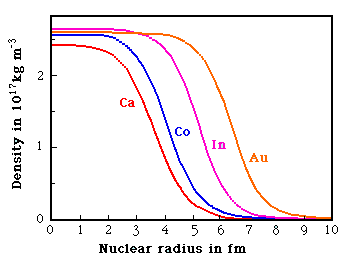
\includegraphics[width=0.5\textwidth]{js10-polomer1.png}}
 \caption{Rozdelenie hustoty pre niektoré jadrá založené na meraniach Hofstadtera et al.}
 \label{js10:polomer1}
\end{figure}
\newline
Zároveň se však ukazuje, že v bezprostřední blízkosti jádra působí na jaderné částice specifické přitažlivé síly - jaderné síly, které pro nabité částice mnohonásobně převyšují coulombovské síly. Je proto rozumné definovat poloměr jádra jako poloměr oblasti, ve které hrají jaderné síly rozhodující roli. K tomu účelu je vhodné popsat interakci částice s jádrem pomocí potenciálu $U(r)$, o němž budeme předpokládat, že je sférický (co ale v skutocnosti nie je), což dobře aproximuje chování většiny jader. Výsledný potenciál bude součtem potenciálů interakce coulombovské $U_c(r)$ a interakce jaderné $U_j(r)$ 
\begin{equation} 
U(r)=U_c(r)+U_j(r).
\end{equation}
Za poloměr jádra $R$ lze pak považovat poloměr oblasti, ve které platí $U_c < U_j$. Schématicky je situace znázorněna na obrázku \ref{js10:polomer2}, kde v pravé části je zachycen průběh potenciálu $U(r)$ pro kladně nabitou částici. V oblasti I převládá odpudivá coulombovská interakce, v oblasti II jaderná interakce. Průsečík potenciálu U s osou r udává poloměr R, který lze považovat za poloměr jádra.
\begin{figure}[h]
 \centerline{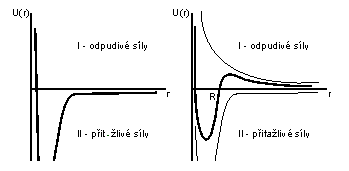
\includegraphics[width=0.5\textwidth]{js10-polomer2.png}}
 \caption{Průběh potenciálu pro neutron (vlevo) a proton v poli jádra.}
 \label{js10:polomer2}
\end{figure}
\newline
První informace o rozměru jader byly získány na základě Rutherfodoveho experimentu, kdy Rutherford ukázal, že při průchodu $\alpha$-částic ve vzdálenosti $L=10-14\,m$ od jádra atomu dochází k narušení coulombovské interakce. Současné výzkumy ukazují, že pro poloměr jader platí dostatečně přesně vztah
$$ R=r_0A^{1/3}, $$
kde A je hmotnostní číslo jádra. Hodnota parametru $r_0$ je $r_0=1,3\times10^{-15}\,m$. Z tohoto vztahu plyne důležitý závěr: objem jádra je přímo úměrný hmotnostnímu číslu A a tedy každý nukleon zaujímá v jádře stejný objem. Lze tedy přibližně interpretovat jádro jako soustavu nukleonů s konstantní hustotou jaderné hmoty. Vhodná parametrická forma jadrovej hustoty bola navrhnuta Woodom a Saxonom 
$$ \rho_N(r)=\frac{\rho_0}{1+e^{\frac{r-R_N}{t}}} $$
kde $t$ je parameter hrúbky povrchu. To je vlastne zobrazene na obrazku \ref{js10:polomer1}.
\section{Hmotnosť atómových jadier}
Hmotnosť jadra je menšia ako súčet hmotností základných nukleónov. Toto odráža skutočnosť, že jadro je viazaný stav castic. Toto vedie k definícii väzbovej energie $E_B$ jadra ako $$  M(A,Z)c^2=Zm_pc^2+(A-Z)m_nc^2-E_B.$$
\section{Väzbová energia jadra}
Väzbová energia je najlepsie popisana Weizsäcker formulou vychadzajuca z Kvapkoveho modelu jadra, ktora ma nasledujuci tvar
$$ E_B=b_vA-b_fA^{2/3}-b_c\frac{Z^2}{A^{1/3}}-b_a\frac{(N-Z)^2}{A}+b_p\delta A^{-3/4} $$
kde $b_v$ a $b_f$ su objemovy a povrchovy clen spojene s tym, ze posobenie nukleonov vo vnutri objemu jadra a na povrchu jadra je rozne. $b_c$ je Coulombicky clen pretoze protony v jadre sa navzajom odpudzuju a to zoslabuje väzbovú energiu jadra. V jadre moze este nastat asymetria medzi poctom protonov a neutronov, ktora taktiez zoslabuje väzbovu energiu. $b_p$ vyjadruje empiricky fakt, ze jadra su silnejsie/slabsie viazane, ak ich pocet protonov alebo neutronov (alebo oboch) je parny/neparny. Odpudzovanie alebo pritahovanie ma nastarosti $\delta$ clen, ktory nadobuda nasledujuce hodnoty:
\begin{itemize}
	\item $\delta=1$ pre even-even jadro
	\item $\delta=0$ pre even-odd jadro
	\item $\delta=-1$ pre odd-odd jadro
\end{itemize}
Posledne dva cleny väzbovej energie vychadzaju zo Shell modelu jadra. Na obrazku \ref{js10:prispevky} su graficky znazornene jednotlive prispevky.\par 
Tieto konštanty boli stanovené empiricky. S týmito 5 konštantami môžme urcit väzbovu energiu pre viac ako 2000 jadier s presnosťou $1-2\%$. Priemerna väzbova energia na jeden nukleon je $$ \epsilon=\frac{E_B}{A}.$$
Pre nazornejsie graficke znazornenie pozri obrazok \ref{js10:vazby}.
\begin{figure}[h]
\begin{subfigure}[b]{0.45\textwidth}
\centering
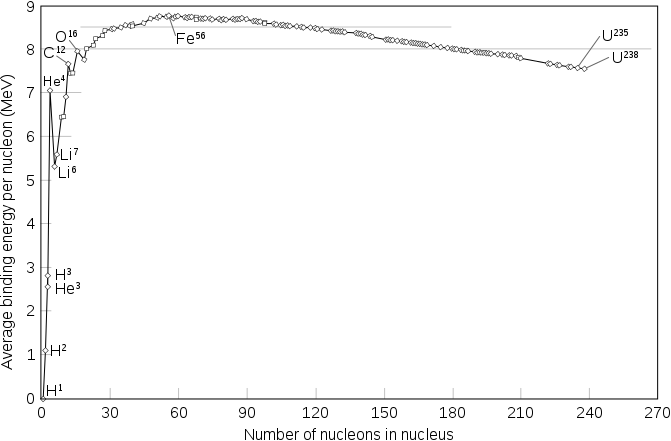
\includegraphics[width=1.0\textwidth]{js10-vazba1.png}
\end{subfigure}
\begin{subfigure}[b]{0.45\textwidth}
\centering
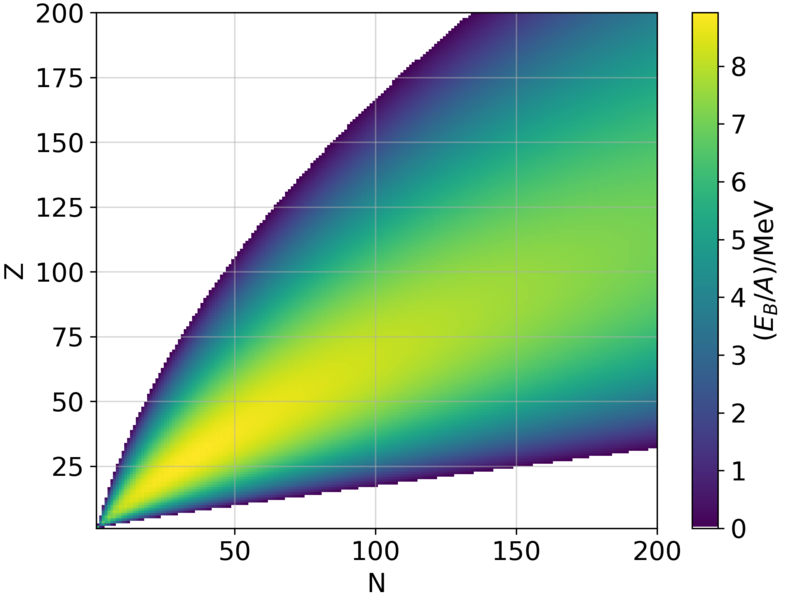
\includegraphics[width=1.0\textwidth]{js10-vazba2.png}
\end{subfigure}
\caption{\textbf{Nalavo:} Krivka väzbovej energie - bežné izotopy. \textbf{Napravo:} Grafické znázornenie semi-empirickej väzbovej energie. Väzbová energia na nukleón v MeV (najvyššie hodnoty sú žltou, viac ako 8,5 MeV na nukleón) je vynesená pre rôzne nuklidy ako funkcia atómového čísla $Z$ (os $y$) počtu neutrónov $N$ (os $x$). Najvyššie hodnoty sú zaznamenané pre $Z=26$ (železo).}
\label{js10:vazby}
\end{figure}
\begin{figure}[h]
 \centerline{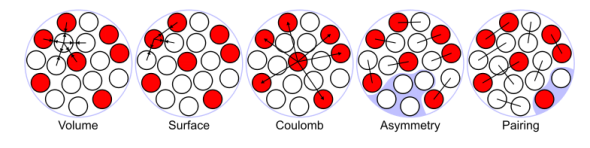
\includegraphics[width=0.8\textwidth]{js10-prispevky.png}}
 \caption{Jednotlive prispevky vazbovej energie.}
 \label{js10:prispevky}
\end{figure}

\section{Parita, moment hybnosti, spin a celkový moment hybnosti}
Jadro je izolovaný systém a tak má dobre definovaný celkovy moment hybnosti ($\vec{J}$), ktory je definovany ako sucet individualnych uhlovych momentov ($\vec{l}$) a spinovych momentov ($\vec{s}$)
\begin{equation}
\vec{J}=\sum_{i=1}^{A}(\vec{l}_i+\vec{s}_i) 
\end{equation}
Tento vektor je jeden zo zakladnych charakteristickych vlastnosti jadroveho stavu. Je potrebné mať na pamäti, že orbitálny moment hybnosti je celočíselným násobkom Planckovej konštanty, zatiaľ čo vnútorny spin nukleónov je polo-číselny nasobok Planckovej konštanty (lebo protony a neutrony su fermiony). Takže parne jadrá majú celočíselné hodnoty pre celkový moment hybnosti a nepárne jadra majú polo-číselné hodnoty celkoveho momentu hybnosti. Všetky jadrá s parnym Z a parnym N majú nulový celkový  moment hybnosti, $\vec{J}=0$. Celkovy moment hybnosti je invariantny vzhladom na rotaciu. \par
Pripomeňme, že parita je spojená s kvantovým číslom $\pm1$, čo je spojené s inverziou priestoru. To znamená, že ak $\Pi$ je operator parity, ktorý pôsobí na kompozitnú vlnovú funkciu jadra $\Psi(\vec{x},A,Z)$
potom 
\begin{equation}
\Pi \Psi(\vec{x},A,Z)=\pm \Psi(-\vec{x},A,Z).
\end{equation}
Znamienko plus je spojene s parnou funkciou a znamienko minus je spojene so neparnou funkciou. Celkovy moment hybnosti a parita su meratelne, na popis sa pouziva notacia $J^{\Pi}$. Napriklad: $^{235}U$ ma $J^{\Pi}=\frac{7}{2}^{-}$, zatial co $^{238}U$ ma $J^{\Pi}=0^{+}$. Na obrazku \ref{js10:spiny} mozme vidiet priklad diskretnych energetickych hladin, ktore su definovane kvantovymi caslami (celkovym momentom hybnosti, paritou etc.)
\begin{figure}[h]
 \centerline{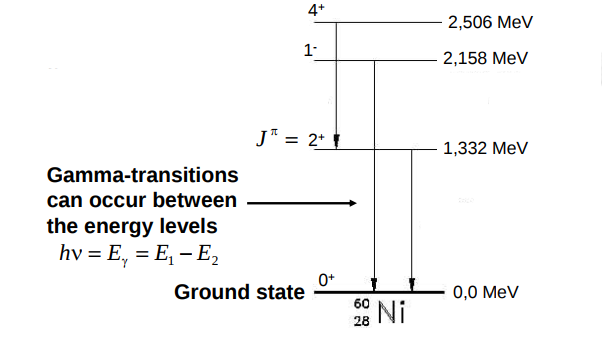
\includegraphics[width=0.6\textwidth]{js10-parita.png}}
 \caption{Energy levels of the $_{28}^{60}Ni$ nucleus.}
 \label{js10:spiny}
\end{figure}
\newline
Parita je dana $\Pi=-1^{(l)}$, kde $l$ je sucet jednotlivych klasickych momentov hybnosti (bacha nie je to celkovy moment hybnosti ani spin).
\section{Jadrový elektrický a magnetický moment}
Statické elektromagnetické vlastnosti jadier sú špecifikované pomocou elektromagnetických momentov, ktoré poskytujú informácie o tom, ako je magnetický moment a náboj distribuovaný v celom jadre. Dva najdolezitejsie momenty su elektricky kvadrupolovy moment (Q) a magneticky dipolovy moment ($\mu$), ktore si teraz predstavime blizsie.
\subsection{Magnetický dipólový moment jadra}
Vieme, ze magnetické polia generované pohyblivými nábojmi majú malý, ale merateľný účinok na energetické hladiny viazaných elektrónov v atóme. Samotné jadro je tvorené protónmi a neutrónmi, ktoré majú svoj vlastny vnútorny spin. Vdaka tomuto spinu si protony a neutrony vytvaraju svoje vlastné \quotedblbase \textit{spinové}\textquotedblright ~magnetické polia, okrem orbitálneho. To poskytuje dodatočný krútiaci moment na elektróneve spiny, čo vedie k \quotedblbase \textit{hyperjemnej strukture}\textquotedblright ~atómovych energetickych hladin. Tieto energetické rozdiely sú malé, ale napriek tomu dôležité pre interpretáciu atómových spektier a preto je dolezite popisat magneticke polia generovane protonmi a neutronmi. Preto sa teraz sustredme na nukleóny v pevne viazanom jadre, kde sa tieto nukleony pohybuju rýchlosťou približne $0,001-0,1\,c$.\par
Jadrové magnetické dipólove momenty vychádzajú z vnútorných spinových magnetických dipólových momentov protónov a neutrónov v jadre a z prúdov cirkulujúcich v jadre kvôli pohybu protónov. Aby sme určili prispevok orbitálneho momentu hybnosti do magnetickeho momentu budeme nukleóny považovat za bodové častice. Pre bodovu casticu mozme pisat 
\begin{equation}
M2=\vec{\mu}=\frac{\mu_N}{\hbar}\sum_{i=1}^A\big( g_l\vec{l_i} + g_s\vec{s_i} \big),
\end{equation}
kde $\mu_N=\frac{e\hbar}{2m_p}\approx5.0507\times 10^{-27}J/T$ je jadrovy magneton, $g_l$ je g-faktor ($g_l=1$ pre proton a $g_l=0$ pre neutron, kedze neutron je neutralny) a $g_s$ je spinovy $g-faktor$ ($g_s=5.5856...$ pre proton, $g_s=-3.8260...$ pre neutron a $g_s=-2.0023...$ pre elektron). Elektronovy $g-faktor$ bol velmi presne predpovedany z $QED$ co vlastne bol velky triumf tejto kvantovej teorie pola.
\subsection{Elektrický kvadrupólový moment jadra}
Závisí od rozloženia náboja vo vnútri jadra a je mierou jadrového tvaru. Elektrostatický potenciál jadra je daný:
\begin{equation}
V(\vec{r})=\frac{1}{4\pi\epsilon_0}\int d\vec{r}^{\prime}\frac{\rho_p({\vec{r}^{\prime}})}{\lvert \vec{r}-\vec{r}^{\prime} \rvert},
\end{equation}
kde 
\begin{equation}
\int \rho_p(\vec{r}^{\prime})d\vec{r}^{\prime}=Ze
\end{equation}
Teraz si predstavme, že skúmame jadro z veľkej vzdialenosti ($r^{\prime} <<< r$), pozri obrazok \ref{js10:potencial}. 
\begin{figure}
 \centerline{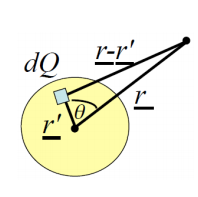
\includegraphics[width=0.2\textwidth]{js10-potenial.png}}
 \caption{Vzajomna poloha vektorov $\vec{r}^{\prime}$ a $\vec{r}$.}
 \label{js10:potencial}
\end{figure}
Za tychto okolnosti mozme dany potencial rozvinut pomocou Taylorovho radu v mocninach $r^{\prime}/r:$
\begin{equation}
V(r)=\frac{1}{4\pi\epsilon_0r} \big[ Ze+\frac{1}{r}\int z \rho(r^{\prime})d\vec{r}^{\prime}+\frac{1}{2r^2}\int(3z^2-r^{\prime2})\rho(r^{\prime})d\vec{r}^{\prime} +... \big] \hspace{0.7cm} kde \hspace{0.7cm} z=r^{\prime}\cos(\theta)
\end{equation}
Z kvantovej mechaniky dalej vieme, ze $ \rho(r^{\prime})=Ze [\psi(\vec{r}^{\prime})\psi^{*}(\vec{r}^{\prime})] $. Elektrické momenty sa oznacuju podla mocniny $1/r$ v zatvorke
\begin{itemize}
	\item \textbf{E0 moment}: elektricky monopol (naboj) $\rightarrow$ $Ze\int \psi^{*}\psi d\vec{r}^{\prime}=Ze$.
	\item \textbf{E1 moment}: elektricky dipol $\rightarrow$ $d=\int \psi^{*}z\psi d\vec{r}^{\prime}$ $\rightarrow$ Bude-li elektrický náboj v jádře rozložen symetricky, lze očekávat, že dipólový moment jádra bude nulový nebo velmi malý. Experimenty ukazují, že pro základní stav jádra je $d=0$, tedy elektrický náboj v jádře je rozložen stejnoměrně. Navyse jadrove vlnove funkcie maju definovanu paritu ako $\lvert \psi(\vec{r}) \rvert^2 = \lvert \psi(-\vec{r}) \rvert^2 \Rightarrow$ elektricky dipolovy moment je vzdy nulovy.
	\item \textbf{E2 moment}: elektricky kvadrupolovy moment $\rightarrow$ $Q=\frac{1}{e} \int (3z^2-r^2)\rho(\vec{r})d\vec{r}$ $\rightarrow$  $Q$ udává odchylku skutečného rozložení náboje od sférického. Elektrický quadrupolový moment jadra opisuje efektívny tvar elipsoidu rozloženia jadrového náboja. Nenulový kvadrupolový moment $Q$ naznačuje, že distribúcia náboja nie je sféricky symetrická. Prvýkrát sa objavil v deuteróne pri pozorovaní \textit{hyperjemnej} štruktúry atómových spektrálnych ciar. Vsetky $J=0$ maju $Q=0$. Ak to ale nie je nulove mozu nastat dva pripady, ktore su znazornene na obrazku \ref{js10:kvadr}
	\begin{figure}[!h]
 	\centerline{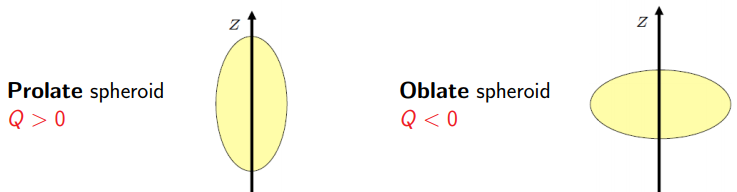
\includegraphics[width=0.8\textwidth]{js10-kvadrupol.png}}
	\caption{Graficke znaornenie kvadrupoloveho momentu.}
 	\label{js10:kvadr}
	\end{figure}
\end{itemize}

Interakční energie elektromagnetickej interakce v jádře je dána elektrickými náboji hadronů a jejich elektrickými proudy (dány pohybem nabitých hadronov (protonov) a magnetickými momenty hadronov (protonov aj neutronov). Tvar hamiltonianu, ktory popisuje danu interakciu je nasledovny
\begin{equation}
H_{elmag}=\int\rho(\vec{r},t)\varphi(\vec{r},t)d\vec{r}-\frac{1}{c}\int\vec{j}(\vec{r},t)\vec{A}(\vec{r},t)d\vec{r},
\end{equation}
kde $\big[ \varphi(\vec{r},t),\vec{A}(\vec{r},t) \big]$ je stvorvektor elektromagnetickeho potencialu a $\big[\rho(\vec{r},t),\frac{\vec{j}}{c}(\vec{r},t)) \big]$ je stvorvektor nabojoveho prudu.\par
Za predpokladu, ze jadro budeme brat ako system bodovych nukleonov mozme pisat 
\begin{itemize}
	\item hustota naboja: $\rho(\vec{r})=\sum_{i=1}^Ae\big( \frac{1}{2}+t_z^i \big)\delta(\vec{r}-\vec{r}_{i})$
	\item hustota prudu: $\vec{j}(\vec{r})=\sum_{i=1}^Ae\big( \frac{1}{2}+t_z^i \big) \frac{1}{2}\big[\vec{v}_i \delta(\vec{r}-\vec{r}_i) + \delta(\vec{r}-\vec{r}_i)\vec{v}_i \big] + \mu_jc\sum_{i=1}^Ag_s^i(\nabla \times \vec{s}_i) \delta(\vec{r}-\vec{r}_i)  $
\end{itemize}
kde $\mu_j$ je jadrovy magneton, a $t_z^i$ je projekcia izospinu (pre proton: $1/2$, pre neutron: $-1/2$) a $g_s^i$ je gyromagneticky pomer alebo inak g-faktor, ktory je vyjadreny nasledovne
$$ g_s^i = \frac{1}{2}g_0-t_z^ig_1 \hspace{0.5cm} kde \hspace{0.5cm} g_0=g_p+g_n \hspace{0.5cm} a \hspace{0.5cm} g_1=g_p-g_n $$

\par
Prvy clen v hustote prudu vznika vdaka pohybu nabitych nukleonov zatial co druhy clen vznika pri interakcii magnetickych momentov nukleonov. Studiom elektromagnetickej interakcie nukleonov mozme studovat rozlozenie naboja v jadre, rychlost, spin alebo izospin nukleonov.\par
Elektromagneticka konstanta jemnej struktury je $\alpha=1/137$. To, ze je taka mala nam umoznuje pouzit poruchove metody $\Rightarrow$ zakony zachovania alebo vyberove pravidla. Predpokladajme, ze mame pripad kde $\varphi=0$ a pole $\vec{A}(\vec{r},t)$ bude splnat Maxwelove rovnice. Spravime multipolovy rozvoj a zavedieme nejake to vyberove pravidlo.\par
Vseobecne plati, ze kazde vektorove pole sa da vyjadrit lubovolnym uplnym systemom ortogonalnych rieseni Maxwelovych rovnic. Po nejakych upravach mozme lubovolne vektorove pole vyjadrit ako 
\begin{equation}
A(\vec{r},t) = \sum_{J,M,P}dkq_k^{JMP}e^{-i\omega t}A_{JM}^P(k,r), 
\end{equation}
kde $P=E$ alebo $P=M$.\par
\textbf{Elektromagnetické prechody a výberové pravidlá}\par
Vdaka prispevkom od elektrickych alebo magnetickych momentov su energeticke hladiny jadra rozvetvene. Ako to uz byva zvykom aj tu dochadza k tomu, ze jadro prechadza do nizsich stavov a tym emituje energiu vo forme gama ziarenia. Prechody medzi energetickymi hladinami, ktore su sposobene prave tymito elektromagnetickymi momentami, sa nazyvaju elektromagneticke prechody. Vo vseobecnosti elektricke (naboj)
ziarenie alebo magneticke (prud, magneticky moment) ziarenie moze byt klasifikovane do multipolov $E\lambda$ alebo $M\lambda$ radu $2^{\lambda}$ ($E1\rightarrow$ elektricky dipol lebo $2^1$). Prechod, kde sa moment hybnosti pociatocneho a koncoveho stavu zmeni, moze nastat prostrednictvom niekolkych multipolovych prechodov, najpravdepodobnejsie sa vsak realizuju najnizsie multipolove prechody ($E1,E2$) alebo ($M1,M2$). Vyemitovana castica odnesie moment hybnosti $\lambda$, pre foton musi platit, ze $\lambda\geq1$, kedze je to vektorova castica ($J^{\Pi}=1^{-}$). Preto prechody $E0$, $M0$ nemozu nastat (navyse magneticky monopol ani neexistuje). Celkovy moment hybnosti sa musi zachovavat a preto pre $\lambda$ musi platit nasledovne
$$ \lvert J_i-J_f \rvert \leq \lambda \leq J_i+J_f $$
$$ J_i=J_f+\lambda,$$
navyse pre paritu musi platit:
\begin{itemize}
	\item Pre elektricky multipolovy prechod $\Pi(E\lambda)=\Pi_i\Pi_f=(-1)^{\lambda}$
	\item Pre magneticky multipolovy prechod $\Pi(M\lambda)=\Pi_i\Pi_f=(-1)^{\lambda+1}$
\end{itemize}
Preto sa parita nemeni pre \textit{E-parne} a \textit{M-neparne} mutipolove prechody zatial co pre \textit{E-neparne} a \textit{M-parne} sa parita nezachovava. Pre ukazku takychto prechodov pozri obrazok \ref{js10:prechody}.
\begin{figure}[!h]
\centerline{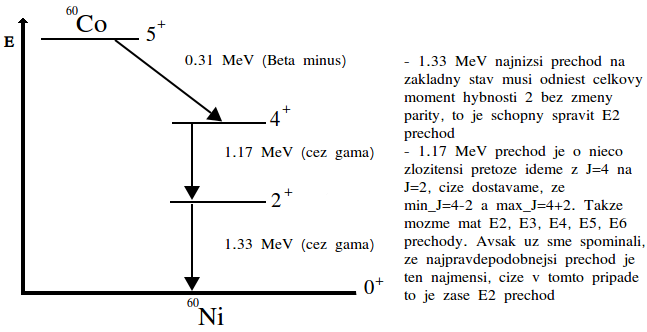
\includegraphics[width=0.9\textwidth]{js10-prechody.png}}
\caption{Schema multipolovych prechodov.}
\label{js10:prechody}
\end{figure}
\newline
Takze, ked to zhrniem pre prechody medzi hladinami so spinom $J_i$ a $J_f$ a paritami $\Pi_i$ a $\Pi_j$ mame:
\begin{itemize}
	\item $J=\lvert J_i-J_f \rvert$ pre $J_i \neq J_f$.
	\item $J=1$ pre $J_i=J_f >0$
	\item Potom dostavame pravidlo: $\Pi_i\Pi_f=(-1)^{J+K}$ kde $K=0$ pre $EJ$ a $K=1$ pre $MJ$
\end{itemize}
To posledne pravidlo sme vlastne uz definovali vyššie ale je dobre ho zopakovat. Navyse z tych obmedzeni vidime, ze prechod s vyziarenim fotonu medzi stavmy $J_i=0$ a $J_f=0$ neexistuje.
\section{Určenie spinových hladín a multipolarity prechodu}
Na experimentalne urcenie spinovych hladin a multipolarity prechodu mozno vyuzit 
\begin{itemize}
	\item Vyuzitie vyberovych pravidiel pre elektromagneticke prechody
	\item Vyuzitie pomerov medzi pravdepodobnostou gama prechodu a vyziarenia konverzneho elektronu. Urcenie konverzneho koeficientu prechodu $\alpha=\frac{N_e}{N_{\gamma}}$. Jednotlive konverzne koeficinety pre jednotlive vrstvy ($\alpha_K$, $\alpha_L$, $\alpha_M$ ...). Konverzne koeficienty rastu s narastom multipolarity prechodu, dalej plati ze $\alpha(M)>\alpha(E)$ a tieto koeficienty rychlo klesaju s energiou prechodu. Tieto vlastnosti mozno pozorovat na obrazku \ref{js10:koef}.
	\begin{figure}[!h]
	\centerline{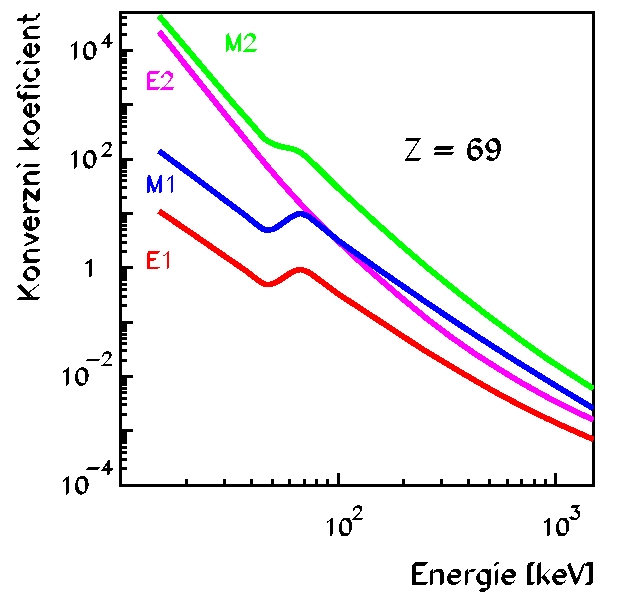
\includegraphics[width=0.4\textwidth]{js10-koenficienty.png}}
	\caption{Koeficienty prechodu.}
	\label{js10:koef}
	\end{figure}
	\item Uhlova korelacia dvoch fotonov vyziarenych za sebou v kaskade.
	\item Udaje o spine z reakcii: analyza priebehu roznych reakcii-rozne reakcie budia hladiny s roznym spinom.
\end{itemize}
\section{Určovanie pravdepodobnosti prechodu z doby života hladín}
\begin{itemize}
	\item Elektronicke metody - meranie krivky rozpadu: meranie izomernych stavov, meranie mimo zvazok ($\tau \sim min-\infty$), transportny system a meranie behom ozarovania ($\tau > \sim s$), meranie na zvazku (celkove rozlisenie radovo v jednotkach az zlomkoch ns). Casove spektrum je tvorene gaussianom (prompt) $+$ exponencialnou krivkou (izomerna). Dosiahnutelna dolna hranica $\tau \sim ns$.
	\item Vyuzitie studia Dopplerovsky posunutej a neposunutej linky v zavislosti na vzdialenosti, v ktorej su odrazene jadra zastavene. Meratelna oblast dob zivota $\tau \sim 10^{-10}- 0^{-12}\,s$.
	\item Metoda zoslabenia Dopplerovho posunu energie ziarenia gama: produckia odrazeneho jadra $\rightarrow$ brzdenie a rozptyl v terci alebo v podlozke $\rightarrow$ vyziareny foton ma rozny Doplerov posun energie $\rightarrow$ zlozity tvar linky. Zo studia tvaru linky sa da urcit doba zivota. Vztah medzi ionizacnymi stratami a drahou je $\Delta x=(dE/dx)^{-1}\Delta E$. Tato metoda ma problemy s popisom brzdenia a mnohonasobneho rozptylu odrazeneho jadra. Meratelna oblast doby zivota je $\tau \sim 10^{-12}-10^{-15}\,s$.
\end{itemize}
\section{Určenie pravdepodobnosti prechodu pomocou Coulombovského budenia}
Vyuzivaju sa zvazky tazkych ionov $\rightarrow$ vysoky naboj $\rightarrow$ budenie stavu s vysokym spinom. Energia zvazku nesmie prekonat energiu Coulombovskej bariery $E_{CB} \sim \frac{Z_1Z_2}{A_1^{-1/3}+A_2^{-1/3}}$, kde $Z_1$, $Z_2$, $A_1$, $A_2$ su parametre nalietavajuceho a tercoveho jadra. Vyhody
\begin{itemize}
	\item cisty elektromagneticky proces
	\item minimalne pozadie
	\item dominantne budenie prostrednictvom $E2$ prechodu 
\end{itemize}
Merane doby zivota $\tau \sim 10^{13}-10^{-9}\,s$.
\section{Štúdium stavov s veľmi vysokým spinom - spiny až $ I\hbar \geq 40\hbar$}
Budenie vysokospinovych stavov v zrazkach tazkych ionov. Po zrazke sa vytvori zlozene jadro ($\tau > 10^{-20}\,s$) - jadra s prebytkom protonov alebo zvazky radioaktivnych jadier (aj jadra s prebytkom neutronov).
Excitacna energia 
$$E_{EX}=E_{CM}+Q,$$ 
kde $Q$ je energia reakcie a $E_{Cm}$ je energia projektilu v CM. Maximalny dosiahnutelny spin je 
$$I^2_{max}=\frac{2\mu R^2}{\hbar^2}(E_{CM}-v_c),$$
kde $\mu$ je redukovana hmotnost a $R$ je najvacsia vzdialenost pri ktorej este vznikne zlozene jadro. Studium tychto stavov umoznuju $4\pi$ multidetektorove spektrometre.\par
Po vzniku zlozeneho jadra sa vypari niekolko nukleonov (prevazne neutrony, lebo su neutralne a tak nemusia prekonat Coulombovsku barieru) $\rightarrow$ rychly ubytok energie ($\sim 8\,MeV/nukleon$) ale len maly ubytok momentu ($\sim 1 \hbar/nukleon$). Tymto procesom konkuruju vysokoenergeticke gama vybijacie giganticke dipolove rozonancie (pretoze nastanu velmi rychlo).\par
\begin{enumerate}
	\item Statisticky zacinaju vo vysokej hustote stavov prechody $E1$ z najvyššie vybudenych stavov.
	\item $E2$ prechody nastavaju blizko Yrast linie.
	\item Pravidelna struktura rotacnych pasov $\sim 1\,MeV$ nad Yrast liniou $\rightarrow$ dostatocna intenzita $\rightarrow$ porovnavanie jednotlivych prechodov.
\end{enumerate}
Yrast linia - spaja stavy s navacsim spinom pre danu energiu. Celkova doba vybijania $\sim 10^{-9}\,s$ s poctom vyziarenych fotonov $\sim 30$. Rozlisujeme tu dva typy rotacie 
\begin{itemize}
	\item Kolektivna rotacia - oblast deformovanych jadier - kolektivny pohyb mnoho neukleonov.
	\item Nekolektivna rotacia - sfericke a slabo deformovane jadra - vysoky spin je dany pohybom niekolkych nukleonov.
\end{itemize}
Pre vysoke spiny nastavaju prechody medzi jednotlivymi druhmi rotacie a to drasticky zmeni tvar jadra. Vysoke spiny $\rightarrow$ rychla rotacia $\rightarrow$ silna Coriolisova interakcia medzi casticovym a rotacnym pohybom $\rightarrow$ krizenie pasov $\rightarrow$ silna Coriolisova interakcia znizuje energiu vybudeneho jednocasticoveho stavu nad ktorym je rozvinuty rotacny pas $\rightarrow$ dochadza k prekryzeniu energetickych pasov.
\section{Superdeformované stavy}
Stavy s velmi vysokou deformaciou (pomer os 2:1 a viac), ktore su predpovedane Shell modelom. Nastavaju pre vysoke spiny $\sim 40-70 \hbar$. Dlhe rotacne pasy vybijane dlhymi kaskadamy $E2$ prechodov.
\section{Gigantické rezonancie}
Vzajomny kolektivny pohyb roznych typov nukleonov, pozri obrazok \ref{js10:gigant},
\begin{itemize}
	\item s roznou orientaciou spinu
	\item s roznou orientaciou izospinu (protonove kvapaliny voci neutronovej)
\end{itemize}
Gigantické rezonance se velmi dobře získávají pomocí Coulombovské excitace.
\begin{figure}[!h]
\centerline{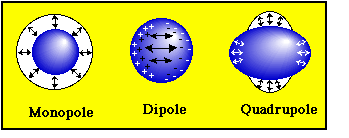
\includegraphics[width=0.5\textwidth]{js10-gignat.png}}
\caption{Rozne typy gigantickych rezonancii.}
\label{js10:gigant}
\end{figure}
Taketo typy rezonancii su studovane napriklad spektrometrom TAPS v GSI Darmstadt.


\end{document}